% This is samplepaper.tex, a sample chapter demonstrating the
% LLNCS macro package for Springer Computer Science proceedings;
% Version 2.20 of 2017/10/04
%
\documentclass[runningheads]{llncs}
%
\usepackage{hyperref}
\usepackage{tikz}
\usepackage{subcaption}
\usepackage{algpseudocode}
\usepackage{algorithm}
\usepackage{stackengine}
\usepackage{amssymb}
\usepackage{caption}

\DeclareCaptionLabelFormat{andtable}{#1~#2  \&  \tablename~\thetable}

\algrenewcommand{\alglinenumber}[1]{\tiny#1:}

% Used for displaying a sample figure. If possible, figure files should
% be included in EPS format.
%
% If you use the hyperref package, please uncomment the following line
% to display URLs in blue roman font according to Springer's eBook style:
\renewcommand\UrlFont{\color{blue}\rmfamily}

\newcommand\specialcaret{%
  \stackengine{0pt}{\ \,}{\scalebox{1.1}[2]{\raisebox{-0.9ex}{\string^}}}{O}{c}{F}{T}{L}}

\begin{document}
%
\title{Generalized Fixed-Depth Prefix and Postfix Symbolic Regression Grammars}%\thanks{Supported by organization x.}}
%
%\titlerunning{Abbreviated paper title}
% If the paper title is too long for the running head, you can set
% an abbreviated paper title here
%
\author{Edward Finkelstein\inst{1}}%\orcidID{}}
%
\authorrunning{Edward F.}
% First names are abbreviated in the running head.
% If there are more than two authors, 'et al.' is used.
%
\institute{Martell, Nebraska, USA\\
\email{edfink234@gmail.com}}
%
\maketitle              % typeset the header of the contribution
%
\begin{abstract}
We develop faultless, fixed-depth, string-based, prefix and postfix symbolic regression grammars, capable of producing \emph{any} expression from a set of operands, unary operators and/or binary operators. Using these grammars, we outline simplified forms of 5 popular heuristic search strategies: Brute Force Search, Monte Carlo Tree Search, Particle Swarm Optimization, Genetic Programming, and Simulated Annealing. For each algorithm, we compare the relative performance of prefix vs postfix for 10 different ground-truth expressions implemented entirely within a common C++/Eigen framework. We find that postfix tends to outperform prefix when the ground-truth expression tree has a larger average number of nodes per layer, and vice versa for prefix when the ground-truth expression tree is relatively thin.

\keywords{symbolic-regression  \and prefix \and postfix.}
\end{abstract}

\section{Introduction}
Symbolic regression (SR) denotes finding a symbolic model $f\left(\vec{x}\right)$ that predicts a label $y$ based on an N-dimensional feature vector $\vec{x}$ while minimizing a loss metric $\mathcal{L}\left(f\left(\vec{x}\right),y\right)$. The search space contains nodes in one of the following classes:
\begin{itemize}
\item \textbf{Unary operators: } Any operator that takes 1 argument as input and outputs a value, such as $\cos$, $\sin$, $\exp$, $\ln$, $\tan$, etc.
\item \textbf{Binary operators: } Any operator that takes 2 arguments as input and outputs a value, such as $+$, $-$, $*$, $\div$, etc.
\item \textbf{Leaf Nodes: } Any of the individual features $\vec{x} = \{x_1, x_2, \ldots,x_{N}\}$ and a constant token that can be optimized with a non-linear optimization routine like L-BFGS \cite{doi:10.1137/0916069} or Levenberg-Marquadt \cite{83b09f23-b20e-3617-8f72-24765b713f7b} \cite{doi:10.1137/0111030}.
\end{itemize}
\subsection{Prefix and Postfix Notation in Symbolic Regression}
\textbf{Pre}fix (also known as Polish notation) expressions are written with the operators coming \emph{before} the operators, for example, \texttt{+ 1 2} represents the sum of 1 and 2. \textbf{Post}fix (also known as Reverse-Polish notation) expressions, on the other hand, have the operators coming \emph{after} the operands, for example, \texttt{1 2 +} represents the sum of 1 and 2. Both prefix and postfix remove the need for parentheses and operator precedence rules characteristic of infix notation (where operators are placed \emph{in between} operands), resulting in faster expression evaluation and less memory. An interesting question then arises: \emph{In symbolic regression, which performs better, prefix or postfix?}
\par To our knowledge, the only paper that studies the effect of prefix vs postfix expressions in SR is \cite{hemberg2008pre}.  In \cite{hemberg2008pre}, the authors compare prefix, infix, and postfix notation-based grammars on 5 bivariate equations and found that postfix performed better than prefix as the complexity increased due to the smaller percentage of invalid individuals.  
Succinctly, the 2 main limitations of \cite{hemberg2008pre} are:
\begin{enumerate}
\item The study does not consider \emph{faultless grammars}, i.e., grammars which do not produce invalids.
\item The study only considers genetic algorithms.
\end{enumerate}
In this paper, we outline faultless grammars for generating fixed-depth prefix and postfix expressions. Additionally, we benchmark the performance of 5 algorithms employing these grammars, namely, Random Search, Monte Carlo Tree Search (MCTS), Particle Swarm Optimization (PSO), Genetic Programming (GP), and Simulated Annealing (SA). 
\par Other papers \cite{lacava2021contemporary}, \cite{10.1145/3205455.3205539}, \cite{Zegklitz2021}, have performed comprehensive comparisons of different SR methods, though usually within the context of different frameworks, which could obscure otherwise very good algorithms by differences in implementation efficiency/speed. Therefore, we implement everything in one common C++ framework utilizing the Eigen template library  \cite{eigenweb}, \href{https://github.com/edfink234/Alpha-Zero-Symbolic-Regression/tree/prefix_and_postfix_cpp_implementation}{here}.

 

\section{Background}\label{sec:Background}
At the core of every SR framework lies a choice of expression representation. For example, Figure \ref {GECCO_Framework_reps} lists the frameworks considered in \cite{defranca2023interpretable} and their underlying expression representations (left) and their frequencies in SR publications over time (right).

% \begin{table}
% \caption{\label{GECCO_Framework_reps}List of SR Frameworks submitted to the 2022 GECCO competition \cite{defranca2023interpretable}, their underlying expression representations, and if the expression representation was stated directly in the cited paper or implied via source-code/references.}


% % \\ The frameworks Bingo, E2E Transformer, QLattice, and Operon state their choice of expression representation directly in the cited papers (namely \cite{10.1145/3520304.3534031}, \cite{kamienny2022endtoend}, \cite{Brolos2021AnAT}, and \cite{10.1145/3377929.3398099}, respectively). PS-Tree does not specify \cite{zhang2022ps} but they use the Deap GP framework \cite{DEAP_JMLR2012} (see \href{https://github.com/hengzhe-zhang/PS-Tree/blob/master/pstree/common\_utils.py\#L4}{here}) which represents expressions with prefix notation. TaylorGP strongly implies prefix notation in the example expression written in section 4.1.1 of their paper \cite{10.1145/3512290.3528757}. In Table 2 of the EQL Paper \cite{pmlr-v80-sahoo18a} they refer to the expressions as ``random graphs,'' and evidence of their acyclicity is given in their Jupyter notebook \href{https://github.com/martius-lab/EQL/blob/master/EQL-DIV-ICML-Python3/Evaluation.ipynb}{here}. GeneticEngine implies prefix usage in section 3.2 of their paper \cite{10.1145/3564719.3568697} (namely, ``Starting with the non-terminal root type $\ldots$''). PySR does not state the expression representation in their paper \cite{cranmer2023interpretable}, but a pre-order traversal of the expression tree is somewhat implied in the Julia source file \href{https://github.com/MilesCranmer/SymbolicRegression.jl/blob/db476a708762c81f46f27f22751f7ff3d1153dc7/src/Equation.jl}{here}. The uDSR framework states pre-order traversal of expression trees for the DSR component in their paper (namely, ``$\ldots$ in the pre-order (depth-first then left-to-right) traversal of the corresponding \emph{expression tree} $\ldots$'' in section 2), and for the GP expression generation, use of the Deap GP framework is shown \href{https://github.com/dso-org/deep-symbolic-optimization/blob/2069d4eda47b0fd6d3e66e0ade9605cd9574b87c/dso/dso/gp/utils.py\#L10}{here} \cite{NEURIPS2022_dbca58f3}. 
% % $\mathrm{GP}_{\mathrm{ZGD}}$ \cite{10.1145/3377930.3390237} somewhat implies a pre-order traversal of expression trees in the C source file \href{https://github.com/grantdick/gpzgd/blob/42e5a1829a0b8a2eb50e116000001f82c770791e/src/gp.c}{here}. NSGA-DCGP states at the beginning of section 2 that ``To represent our functional programs we use the Cartesian Genetic Programming framework,'' \cite{izzo2016differentiable}  and the paper they cite directly states ``In CGP, programs are represented in the form of directed acyclic graphs'' \cite{Miller2011}.} 
% \begin{tabular*}{\textwidth}{lll} %open PhD_Papers/2304.01117.pdf 
% \hline
% Framework&Expression Representation & Stated Directly or Implied\\
% \hline
% Bingo \cite{10.1145/3520304.3534031} &Acyclic Graph & Stated Directly\\ %Specified in Paper
% E2E Transformer \cite{kamienny2022endtoend} &prefix & Stated Directly\\ %Specified in Paper
% PS-Tree \cite{zhang2022ps} &prefix & Implied \\ %Not directly specified in Paper, but they use Deap GP (see here: https://github.com/hengzhe-zhang/PS-Tree/blob/master/pstree/common_utils.py#L4) which uses prefix notation internally (Simone said so)
% QLattice \cite{Brolos2021AnAT} & Acyclic Graph & Stated Directly\\ %Specified in Paper
% TaylorGP \cite{10.1145/3512290.3528757} & prefix & Implied \\ %Not directly specified, but they strongly imply it by writing examples in prefix notation in section 4.1.1 of the paper here: https://arxiv.org/pdf/2205.09751.pdf
% EQL \cite{pmlr-v80-sahoo18a} & Acyclic Graph & Implied\\%Table 2 refers to the expressions as ``random graphs,'' and the following Jupyter notebook gives further evidence for this: https://github.com/martius-lab/EQL/blob/master/EQL-DIV-ICML-Python3/Evaluation.ipynb
% GeneticEngine \cite{10.1145/3564719.3568697} & prefix & Implied \\ %'' Starting with the non-terminal
% %root type, a concrete subclass is non-deterministically selected, and that object is created. For each field (or constructor argument), a compatible object is constructed by recursively calling this algorithm. The base case is when native
% %types (like int or float) are used, and then native random
% %value generators are used.'' (section 3.2 ``Meta-handlers'')  
% Operon \cite{10.1145/3377929.3398099} & postfix  & Stated Directly \\ %Specified in Paper
% PySR \cite{cranmer2023interpretable} & prefix & Implied \\%Very characteristic Pre-order traversal of Binary Tree: https://github.com/MilesCranmer/SymbolicRegression.jl/blob/db476a708762c81f46f27f22751f7ff3d1153dc7/src/Equation.jl
% uDSR \cite{NEURIPS2022_dbca58f3} & prefix & Implied \\ %For the DNN part it is stated ``in the pre-order (depth-first then left-to-right) traversal of the corresponding expression'' and the GP part uses deap (see here: https://github.com/dso-org/deep-symbolic-optimization/blob/2069d4eda47b0fd6d3e66e0ade9605cd9574b87c/dso/dso/gp/utils.py#L10)
% $\mathrm{GP}_{\mathrm{ZGD}}$ \cite{10.1145/3377930.3390237} & prefix & Implied\\ %Implied, as init_tree builds expressions by adding operators further down (pre-order) and connects the new pointer by pointing the parent to the current tree
% NSGA-DCGP \cite{izzo2016differentiable} & Acyclic Graph & Implied \\%``To represent our functional programs we use the Cartesian Genetic Programming framework'' which states ``In CGP, programs are represented in the form of directed acyclic graphs'' \cite{Miller2011}
% \hline 
% \end{tabular*}
% \end{table}

\begin{figure}[ht]

    \caption{Left: List of SR Frameworks submitted to the 2022 GECCO competition \cite{defranca2023interpretable}, their underlying expression representations, and if the expression representation was stated directly in the cited paper or implied via source-code/references. Right: Number of SR publications mentioning prefix, postfix, and acyclic graphs over time. The script to reproduce the plot is \href{https://github.com/edfink234/Alpha-Zero-Symbolic-Regression/blob/b2f7486b0797843ee363b20faa9a30677065f7b9/Figure_1/notations_pubs_counter.py}{here}.}
    \centering
    \subfloat{
    \label{GECCO_Framework_reps}
        \scalebox{0.68}{\begin{tabular*}{0.81\textwidth}{l@{\hskip 0.4in}l@{\hskip 0.4in}l} %open PhD_Papers/2304.01117.pdf 
\hline
\textbf{Framework}&\textbf{Representation} & \textbf{Deduced}\\[0.1cm]
\hline
Bingo \cite{10.1145/3520304.3534031} &Acyclic Graph & Stated Directly\\ %Specified in Paper
E2E Transformer \cite{kamienny2022endtoend} &prefix & Stated Directly\\ %Specified in Paper
PS-Tree \cite{zhang2022ps} &prefix & Implied \\ %Not directly specified in Paper, but they use Deap GP (see here: https://github.com/hengzhe-zhang/PS-Tree/blob/master/pstree/common_utils.py#L4) which uses prefix notation internally (Simone said so)
QLattice \cite{Brolos2021AnAT} & Acyclic Graph & Stated Directly\\ %Specified in Paper
TaylorGP \cite{10.1145/3512290.3528757} & prefix & Implied \\ %Not directly specified, but they strongly imply it by writing examples in prefix notation in section 4.1.1 of the paper here: https://arxiv.org/pdf/2205.09751.pdf
EQL \cite{pmlr-v80-sahoo18a} & Acyclic Graph & Implied\\%Table 2 refers to the expressions as ``random graphs,'' and the following Jupyter notebook gives further evidence for this: https://github.com/martius-lab/EQL/blob/master/EQL-DIV-ICML-Python3/Evaluation.ipynb
GeneticEngine \cite{10.1145/3564719.3568697} & prefix & Implied \\ %'' Starting with the non-terminal
%root type, a concrete subclass is non-deterministically selected, and that object is created. For each field (or constructor argument), a compatible object is constructed by recursively calling this algorithm. The base case is when native
%types (like int or float) are used, and then native random
%value generators are used.'' (section 3.2 ``Meta-handlers'')  
Operon \cite{10.1145/3377929.3398099} & postfix  & Stated Directly \\ %Specified in Paper
PySR \cite{cranmer2023interpretable} & prefix & Implied \\%Very characteristic Pre-order traversal of Binary Tree: https://github.com/MilesCranmer/SymbolicRegression.jl/blob/db476a708762c81f46f27f22751f7ff3d1153dc7/src/Equation.jl
uDSR \cite{NEURIPS2022_dbca58f3} & prefix & Implied \\ %For the DNN part it is stated ``in the pre-order (depth-first then left-to-right) traversal of the corresponding expression'' and the GP part uses deap (see here: https://github.com/dso-org/deep-symbolic-optimization/blob/2069d4eda47b0fd6d3e66e0ade9605cd9574b87c/dso/dso/gp/utils.py#L10)
$\mathrm{GP}_{\mathrm{ZGD}}$ \cite{10.1145/3377930.3390237} & prefix & Implied\\ %Implied, as init_tree builds expressions by adding operators further down (pre-order) and connects the new pointer by pointing the parent to the current tree
NSGA-DCGP \cite{izzo2016differentiable} & Acyclic Graph & Implied \\%``To represent our functional programs we use the Cartesian Genetic Programming framework'' which states ``In CGP, programs are represented in the form of directed acyclic graphs'' \cite{Miller2011}
\hline 
\end{tabular*}}}
\subfloat
{
    \raisebox{-.5\height}{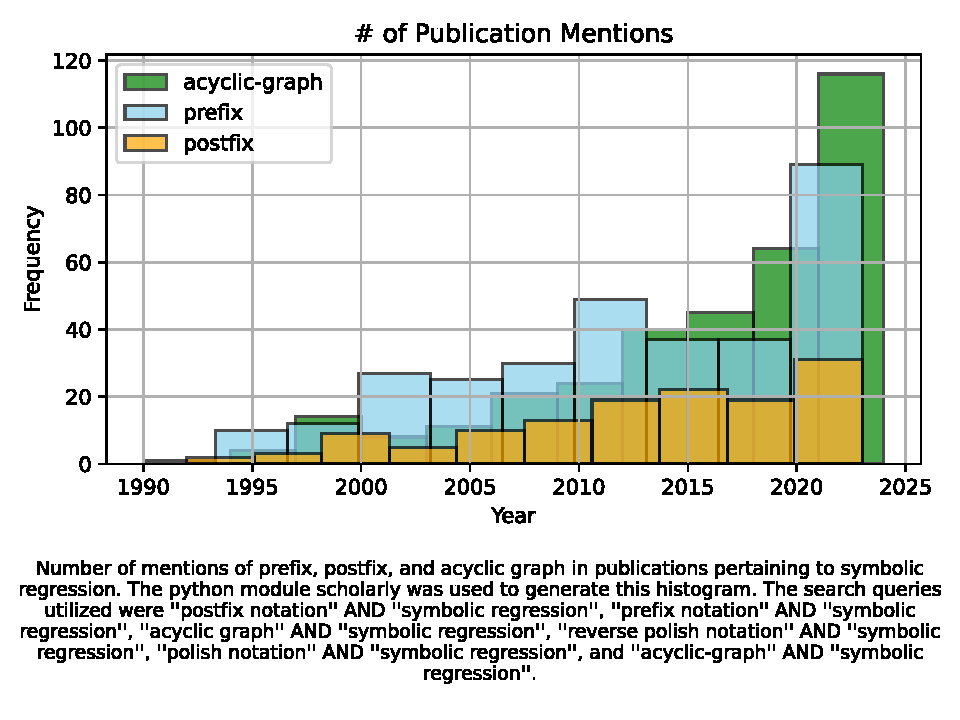
\includegraphics[width=0.43\linewidth]{pub_freqs.pdf}}
    \label{fig:pub_freqs_pre_post_acyc_graph}
}
\end{figure}

Prefix notation and acyclic graphs are generally preferred over postfix notation for representing expressions\footnote{See Figure \ref{fig:pub_freqs_pre_post_acyc_graph} for an illustration \cite{cholewiak2021scholarly}} \cite{defranca2023interpretable}, as they allow for a natural termination condition and reduce the memory required to represent expressions with identical sub-components, respectively. The analysis in this paper is limited to prefix and postfix notations due to their similarity.

 

% Figure \ref{fig:pub_freqs_pre_post_acyc_graph} shows a histogram of publication frequencies mentioning these representations in the context of symbolic regression throughout the years, obtained with the help of the scholarly python module \cite{cholewiak2021scholarly}.  %code here: 
% \begin{figure}[ht]
%     \centering
%     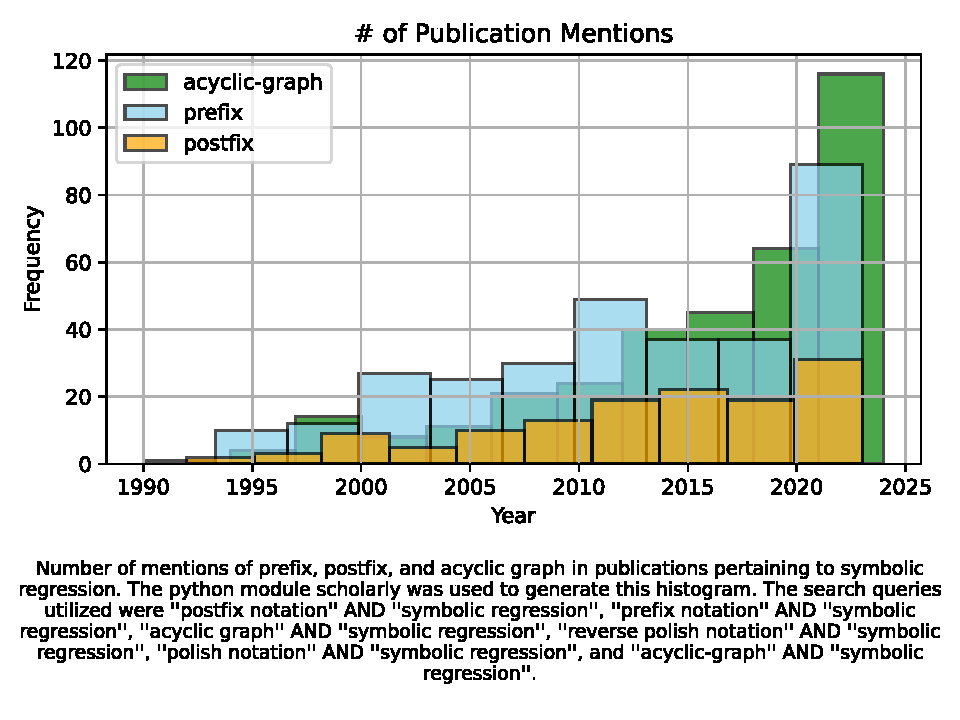
\includegraphics[width=\linewidth]{pub_freqs.pdf}
%     \caption{Number of mentions of prefix, postfix, and acyclic graph in publications pertaining to symbolic regression. The python module scholarly was used to generate this histogram \cite{cholewiak2021scholarly}. The search queries utilized were ``postfix notation'' AND ``symbolic regression'', ``prefix notation'' AND ``symbolic regression'', ``acyclic graph'' AND ``symbolic regression'', ``reverse polish notation'' AND ``symbolic regression'', ``polish notation'' AND ``symbolic regression'', and ``acyclic-graph'' AND ``symbolic regression''. The script to reproduce this plot is \href{https://github.com/edfink234/Alpha-Zero-Symbolic-Regression/blob/d5ebdf90c0915cd5769b29bf679709dbd4a618c7/Figure_1/notations_pubs_counter.py}{here}.} 
%     \label{fig:pub_freqs_pre_post_acyc_graph}
% \end{figure}

\subsection{Prefix and Postfix}
Prefix notation entails building expressions from root nodes, while postfix notation begins expressions from leaf nodes. Figure \ref{fig:prefix_vs_postfix} illustrates the difference.

\begin{figure}[ht]
    \begin{subfigure}[b]{0.4\textwidth}
        \centering
        \begin{tikzpicture}
            \node[text width = 6 cm, align = center] at (0,0) {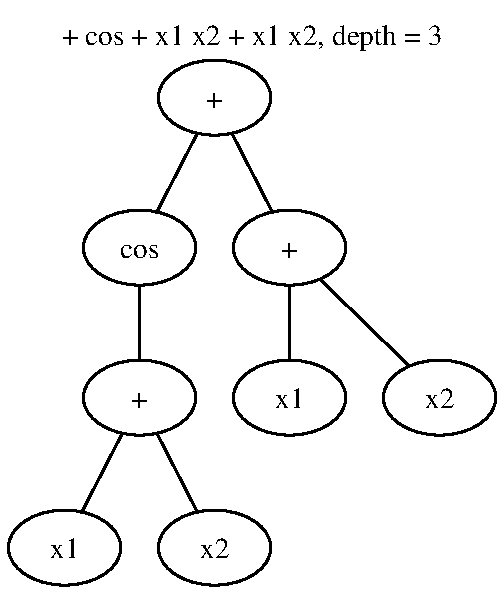
\includegraphics[width=\linewidth, keepaspectratio]
            {expression_tree_PN.pdf}};
            \node at (-1.35, 2.4) {\textcolor{red}{\textbf{1}}};
            \node at (-2.25, 0.6) {\textcolor{red}{\textbf{2}}};
            \node at (-2.25, -1.2) {\textcolor{red}{\textbf{3}}};
            \node at (-3.15, -3) {\textcolor{red}{\textbf{4}}};
            \node at (-1.325, -3) {\textcolor{red}{\textbf{5}}};
            \node at (-0.4, 0.6) {\textcolor{red}{\textbf{6}}};
            \node at (-0.4, -1.2) {\textcolor{red}{\textbf{7}}};
            \node at (1.4, -1.2) {\textcolor{red}{\textbf{8}}};
        \end{tikzpicture} 
        \caption{prefix}
        \label{subfig:prefix_tree_example}
    \end{subfigure}
    \hspace{1cm}
    \begin{subfigure}[b]{0.4\textwidth}
        \centering
        \begin{tikzpicture}
            \node[text width = 6 cm, align = center] at (0,0) {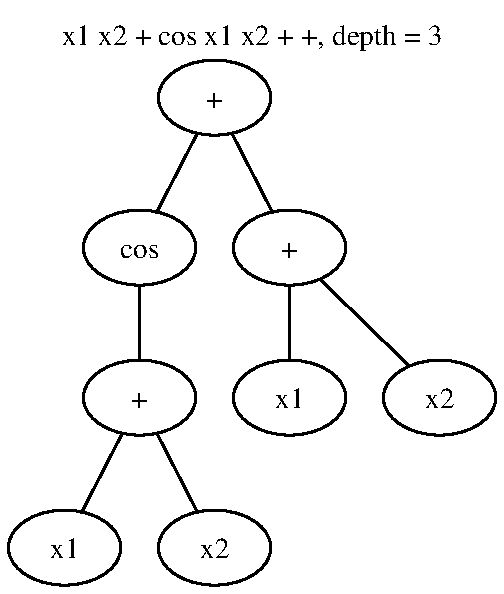
\includegraphics[width=\linewidth, keepaspectratio]{expression_tree_RPN.pdf}};
            \node at (-1.35, 2.4) {\textcolor{red}{\textbf{8}}};
            \node at (-2.25, 0.6) {\textcolor{red}{\textbf{4}}};
            \node at (-2.25, -1.2) {\textcolor{red}{\textbf{3}}};
            \node at (-3.15, -3) {\textcolor{red}{\textbf{1}}};
            \node at (-1.325, -3) {\textcolor{red}{\textbf{2}}};
            \node at (-0.4, 0.6) {\textcolor{red}{\textbf{7}}};
            \node at (-0.4, -1.2) {\textcolor{red}{\textbf{5}}};
            \node at (1.4, -1.2) {\textcolor{red}{\textbf{6}}};
        \end{tikzpicture}
        \caption{postfix} \label{subfig:postfix_tree_example}
    \end{subfigure}
    \caption{Prefix \& postfix representation of the infix expression $f(x_1, x_2) = \cos(x_1 + x_2) + (x_1 + x_2)$. The numbers \textcolor{red}{\textbf{1}} - \textcolor{red}{\textbf{8}} denote the order of tokens.}
    \label{fig:prefix_vs_postfix}
\end{figure}

\par Prefix notation disables expansion of a completed expression tree branch without modifying a leaf node. Contrarily, postfix notation allows the tree to expand upwards from the root node, see, e.g., $\textbf{\textcolor{red}{3}} \rightarrow \textbf{\textcolor{red}{4}} $ in Figure \ref{subfig:postfix_tree_example}.

% \begin{figure}[ht]
%     \begin{subfigure}[b]{0.51\textwidth}
%         \centering
%         \begin{tikzpicture}
%             \node[text width = 6 cm, align = center] at (0,0) {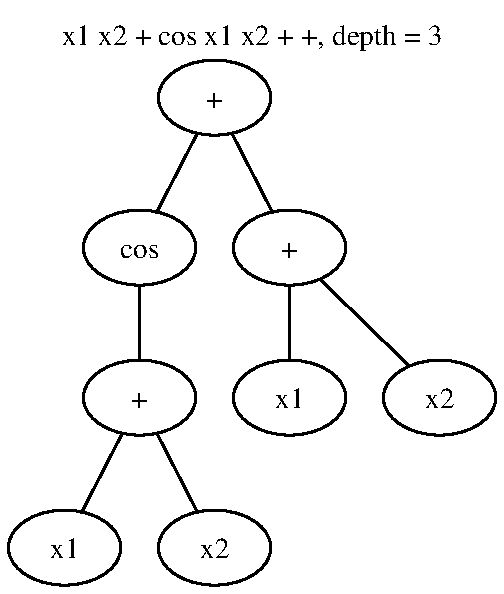
\includegraphics[width=\linewidth, keepaspectratio]{expression_tree_RPN.pdf}};
%             \node at (-1.35, 2.4) {\textcolor{red}{\textbf{8}}};
%             \node at (-2.25, 0.6) {\textcolor{red}{\textbf{4}}};
%             \node at (-2.25, -1.2) {\textcolor{red}{\textbf{3}}};
%             \node at (-3.15, -3) {\textcolor{red}{\textbf{1}}};
%             \node at (-1.325, -3) {\textcolor{red}{\textbf{2}}};
%             \node at (-0.4, 0.6) {\textcolor{red}{\textbf{7}}};
%             \node at (-0.4, -1.2) {\textcolor{red}{\textbf{5}}};
%             \node at (1.4, -1.2) {\textcolor{red}{\textbf{6}}};
%         \end{tikzpicture}
%         \caption{postfix (before)}
%     \end{subfigure}
%     \hspace{1cm}
%     \begin{subfigure}[b]{0.51\textwidth}
%         \centering
%         \begin{tikzpicture}
%             \node[text width = 6 cm, align = center] at (0,0) {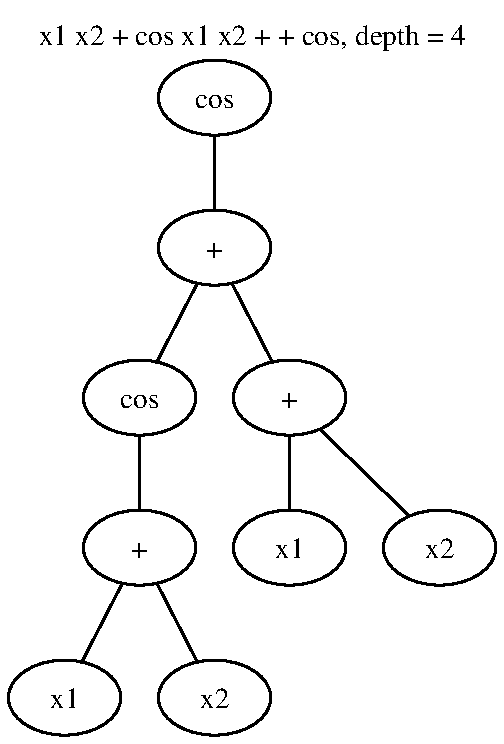
\includegraphics[width=\linewidth, keepaspectratio]{expression_tree_1_RPN.pdf}};
%             \node at (-1.35, 3.3) {\textcolor{red}{\textbf{9}}};
%             \node at (-1.35, 1.5) {\textcolor{red}{\textbf{8}}};
%             \node at (-2.25, -0.3) {\textcolor{red}{\textbf{4}}};
%             \node at (-2.25, -2.1) {\textcolor{red}{\textbf{3}}};
%             \node at (-3.15, -3.9) {\textcolor{red}{\textbf{1}}};
%             \node at (-1.325, -3.9) {\textcolor{red}{\textbf{2}}};
%             \node at (-0.4, -0.3) {\textcolor{red}{\textbf{7}}};
%             \node at (-0.4, -2.1) {\textcolor{red}{\textbf{5}}};
%             \node at (1.4, -2.1) {\textcolor{red}{\textbf{6}}};
%         \end{tikzpicture}
%         \caption{postfix (after)}
%     \end{subfigure}
%     \caption{Adding a node to a postfix expression tree from left (node \textcolor{red}{\textbf{8}}) to right (node \textcolor{red}{\textbf{9}}). As one can see, even though the expression on the left is complete, the tree can grow using the same method. This is not the case for the prefix representation. For example, to continue the expression tree in Figure \ref{subfig:prefix_tree_example}, one would have to add nodes going up from the root.}
%     \label{fig:postfix_add_1}
% \end{figure}

\subsection{Building Fixed-Depth Expressions}
Building fixed-depth prefix or postfix expressions requires determining the legal nodes at each step. 
\par At each step, a ``token" is added to an array. The set of selectable nodes at a given step ensures that any \emph{valid} expression can be generated with depth $N$. Tokens are appended left-to-right as they appear in prefix or postfix notation. 
\par The set of legal tokens at each step consists of unary operators and/or binary operators and/or leaf nodes of sizes $N_U$, $N_B$, and  $N_L$, respectively. $N_{T} = N_U + N_B + N_L$ denotes the total number of tokens considered. Determining which nodes are allowed in the current step depends on if the expression is prefix or postfix, explained in the remainder of this section.
\subsection{Prefix Grammar}\label{subsec:prefix_grammar}
In the first step, if the specified depth $N=0$, then the allowed tokens are the leaf nodes of size $N_L$, else, they're the operators of size $N_U + N_B$.
\par At each subsequent step, the set of allowed tokens is determined as follows:
\begin{itemize}
    \item \textbf{Unary Operators: }
    Any considered unary operator is valid if adding a unary operator to the current expression can yield an expression with depth $\leq$ the specified depth $N$. Otherwise, a unary operator is not allowed.
    \item \textbf{Binary Operators:}
    Any considered binary operator is valid if adding a binary operator to the current expression can yield an expression with depth $\leq$ the specified depth $N$. Otherwise, a binary operator is not allowed.
    \item \textbf{Leaf Nodes: }
    Any considered leaf node is valid if \emph{both} of the following conditions are false:
    \begin{enumerate}
    \item The current expression has \texttt{num\_leaves = num\_binary - 1}.
    \item Adding a leaf node results in the minimum depth being $<$ the desired depth $N$ \textbf{and} \texttt{num\_leaves = num\_binary} in the current expression.
    \end{enumerate}
\end{itemize}

\subsection{Postfix Grammar}\label{subsec:postfix_grammar}
In the first step, the only allowed tokens are the leaf nodes of size $N_L$.
\par At each subsequent step, the set of allowed tokens is determined as follows:
\begin{itemize}
\item \textbf{Unary Operators: }
Any considered unary operator is valid if $\texttt{num\_leaves} \geq 1$ \textbf{and} if adding a unary operator to the current expression can yield an expression with depth $\leq$ the specified depth $N$. Otherwise, a unary operator is not allowed. 
\item \textbf{Binary Operators: }
Any considered binary operator is valid if $\texttt{num\_binary} \neq \texttt{num\_leaves} - 1$ in the current expression. Otherwise, a binary operator is not allowed.
\item \textbf{Leaf Nodes: }
Any considered leaf node is valid if adding a leaf node results in the minimum depth of the expression being $\leq$ the desired depth $N$. Otherwise, a leaf node is not allowed.
\end{itemize}

\subsection{Conclusion}
Evidently, the postfix grammar is simpler than the prefix grammar. The main reason for this difference is that, in prefix notation, one must \emph{additionally} ensure the expression does not complete until it reaches the desired depth $N$. \par One can determine the minimum depth and completeness of a prefix/postfix token array via the stack-based approaches shown \href{https://github.com/edfink234/Alpha-Zero-Symbolic-Regression/blob/0b5b6d0b56c2d108dda023a337edeb1084436da7/PrefixPostfixSR.cpp#L393-L485}{here} and \href{https://github.com/edfink234/Alpha-Zero-Symbolic-Regression/blob/0b5b6d0b56c2d108dda023a337edeb1084436da7/PrefixPostfixSR.cpp#L487-L641}{here}, respectively\footnote{The functions \texttt{getPNDepth} and \texttt{getRPNDepth} come from \cite{77180279} and \cite{77128902}, respectively.}.

% \begin{algorithm}
% \scriptsize
% \caption{Calculate Depth and Completeness of \textbf{Polish Notation (PN)} expressions. Algorithm from \cite{77180279}.}
% \label{alg:getPNdepth}
% \hspace*{\algorithmicindent} \textbf{input:}  expression, expression list of tokens in prefix notation \\
% \hspace*{\algorithmicindent} \textbf{output:} Depth of expression\\
% \hspace*{\algorithmicindent} \textbf{output:} If expression is complete 
% \begin{algorithmic}[1] 
% \Function{getPNdepth}{expression}  %code here
%     \If{expression is empty}
%         \State \Return 0, \textbf{False}
%     \EndIf

%     \State Initialize empty stack
%     \State Initialize depth, numBinary, and numLeaves to 0

%     \For{token \textbf{in} expression}
%         \If{token is binary operator}
%             \State Push 2 onto stack   \Comment\texttt{{Number of operands for binary operators}}
%             \State numBinary $\gets$ numBinary+1
%         \ElsIf{token is unary operator} 
%             \State Push 1 onto stack  \Comment\texttt{{Number of operands for unary operators}}
%         \Else  \Comment\texttt{{An operand}}
%             \State numLeaves $\gets$ numLeaves+1
%             \While{stack is not empty \textbf{and} top of stack == 1}
%                 \State Pop top of stack \Comment\texttt{{Remove fulfilled unary operators}}
%             \EndWhile
%             \If{stack is not empty}
%                 \State Decrement top of stack by 1 \Comment\texttt{{Indicate operand is consumed}}
%             \EndIf
%         \EndIf
%         \State  depth $\gets$ max(depth, stack length + 1)
%     \EndFor
%     \State \Return depth - 1, numLeaves == numBinary + 1 
% \EndFunction
% \end{algorithmic}
% \end{algorithm}

% \begin{algorithm}
% \scriptsize
% \caption{Calculate Depth and Completeness of \textbf{Reverse Polish Notation (RPN)} expressions.  Algorithm from \cite{77128902}.}
% \label{alg:getRPNdepth}
% \hspace*{\algorithmicindent} \textbf{input:}  expression, expression list of tokens in postfix notation \\
% \hspace*{\algorithmicindent} \textbf{output:} Depth of expression\\
% \hspace*{\algorithmicindent} \textbf{output:} If expression is complete 
% \begin{algorithmic}[1]
% \Function{getRPNdepth}{expression} %code here
%     \If{expression is empty}
%         \State \Return 0, \textbf{False}
%     \EndIf

%     \State Initialize empty stack

%     \For{token \textbf{in} expression}
%         \If{token is unary operator} \Comment\texttt{{All unary operators}}
%             \State Increment top of stack by 1 
%         \ElsIf{token is binary operator} \Comment\texttt{{All binary operators}}
%             \State Push max(stack.pop(), stack.pop()) + 1 onto stack 
%         \Else  \Comment\texttt{{All operands}}
%             \State Push 1 onto stack
%         \EndIf
%     \EndFor

%    \If{size of stack greater than 1}

% 	    \While{size of stack greater than 1}
% 	        \State Push max(stack.pop(), stack.pop()) + 1 onto  stack
% 	    \EndWhile
%  	\State \Return stack.pop() - 1, \textbf{False}
    
%     \Else
%     	\State \Return stack.pop() - 1, \textbf{True}
%     	    \EndIf
% \EndFunction
% \end{algorithmic}
% \end{algorithm}

The next section explains the symbolic regression algorithms used in this paper in the context of the fixed-depth grammars developed in this section.

\section{Symbolic Regression Algorithms}\label{sec:SymbolicRegressionAlgorithms}

This section details the fixed-depth-grammar algorithms of this paper: Random Search, Monte Carlo Tree Search (MCTS), Particle Swarm Optimization (PSO), Genetic Programming (GP), and Simulated Annealing (SA).

\subsection{Random Search}\label{subsec:RandomSearch}

Random Search, i.e., the brute-force approach, has gained more attention recently \cite{Heule2017TheSO} as it can rival GP if used with a restrictive grammar \cite{Kammerer2020} or sophisticated search strategy \cite{udrescu2020ai}.
Our random-search approach is as follows:
\par First, one starts with an empty expression list. Then, random \emph{legal} tokens are appended to the expression list until complete with depth $N$, after which the constant tokens (if any) are initialized to 1, optimized with 5 iterations of Levenberg-Marquadt, and cached as initial seeds in case the depth-$N$ expression is re-encountered. Finally, the score of the expression is computed as:

\begin{equation}
\mathrm{Score} = \frac{1}{1+ 1/N_{\mathrm{dat}}\left|\left|\hat{Y}-\vec{Y}\right|\right|^2} \qquad  (0 \leq \mathrm{Score} \leq 1), \label{eq:score_formula}
\end{equation}

where $N_{\mathrm{dat}}$ is the number of data points, $\hat{Y}$ are the predicted labels, and $\vec{Y}$ are the true labels.

% \begin{algorithm}
% \scriptsize
% \caption{Calculate Depth and Completeness of \textbf{Polish Notation (PN)} expressions \cite{77180279}.}
% \label{alg:getPNdepth_cache}
% \hspace*{\algorithmicindent} \textbf{input:}  expression, expression list of tokens in prefix notation \\
% \hspace*{\algorithmicindent} \textbf{input:}  modify, if params should be modified \\
% \hspace*{\algorithmicindent} \textbf{input:}  binary, if depth \& completeness should be determined with binary op.  \\
% \hspace*{\algorithmicindent} \textbf{input:}  unary, if depth \& completeness should be determined with unary op.  \\
% \hspace*{\algorithmicindent} \textbf{input:} leaf, if depth \& completeness should be determined with leaf node \\
% \hspace*{\algorithmicindent} \textbf{output:} Depth of expression\\
% \hspace*{\algorithmicindent} \textbf{output:} If expression is complete \\
% \hspace*{\algorithmicindent} \textbf{param:} stack, the stack used in the algorithm \\
% \hspace*{\algorithmicindent} \textbf{param:} idx, the index of the expression element to use in the computation\\
% \hspace*{\algorithmicindent} \textbf{param:} numBinary, the number of binary operators in the expression \\
% \hspace*{\algorithmicindent} \textbf{param:} numLeaves, the number of leaf nodes in the expression 
% \begin{algorithmic}[1]

% \Function{getPNdepth}{expression, modify = \textbf{False},  binary = \textbf{False},  unary = \textbf{False},  leaf = \textbf{False}}  %code here
%     \If{expression is empty}
%         \State \Return 0, \textbf{False}
%     \EndIf

%     \If{not modify} \Comment\texttt{{called when determining legal tokens}}
%         \If{binary}  %\Comment\texttt{{depth, completeness of PN expression + binary op.}}
%             \State \Return max(depth, stack length + 2) -1,  numLeaves == numBinary + 2
%          \ElsIf{unary}  %\Comment\texttt{{depth, completeness of PN expression + unary op.}}
%             \State \Return max(depth, stack length + 2) -1,  numLeaves == numBinary + 1
%          \ElsIf{leaf}  %\Comment\texttt{{depth, completeness of PN expression + leaf node}}
%             \State lastIdxNot1 $\gets$ index of last element in stack $\neq$ 1
%             \State \Return max(depth, lastIdxNot + 1) -1,  numLeaves == numBinary
%         \EndIf
%     \Else \Comment\texttt{{called after legal token selected}}
%         \If{expression[idx] is binary operator}
%             \State Push 2 onto stack   \Comment\texttt{{Number of operands for binary operators}}
%             \State numBinary $\gets$ numBinary+1
%         \ElsIf{expression[idx] is unary operator} 
%              \State Push 1 onto stack  \Comment\texttt{{Number of operands for unary operators}}
%         \Else  \Comment\texttt{{An operand}}
%             \State numLeaves $\gets$ numLeaves+1
%             \While{stack not empty \textbf{and} top of stack is 1}
%                 \State Pop top of stack \Comment\texttt{{Remove fulfilled unary operators}}
%             \EndWhile
%             \If{stack not empty}
%                 \State Decrement top of stack by 1 \Comment\texttt{{Indicate operand is consumed}}
%             \EndIf
%         \EndIf
%         \State  depth $\gets$ max(depth, stack length + 1)
%         \State idx $\gets$ idx + 1
%     \EndIf
%     \State \Return depth - 1, numLeaves == numBinary + 1 
% \EndFunction
% \end{algorithmic}
% \end{algorithm}

% \begin{algorithm}
% \scriptsize
% \caption{Calculate Depth and Completeness of \textbf{Reverse Polish Notation (RPN)} expressions \cite{77128902}.}
% \label{alg:getRPNdepth_cache}
% \hspace*{\algorithmicindent} \textbf{input:}  expression, list of tokens in postfix notation \\
% \hspace*{\algorithmicindent} \textbf{input:}  modify, if params should be modified \\
% \hspace*{\algorithmicindent} \textbf{input:}  unary, if depth \& completeness should be determined with unary op.  \\
% \hspace*{\algorithmicindent} \textbf{input:} leaf, if depth \& completeness should be determined with leaf node \\
% \hspace*{\algorithmicindent} \textbf{output:} Depth of expression\\
% \hspace*{\algorithmicindent} \textbf{output:} If expression is complete \\
% \hspace*{\algorithmicindent} \textbf{param:} stack, the stack used in the algorithm \\
% \hspace*{\algorithmicindent} \textbf{param:} idx, the index of the expression element to use in the computation
% \begin{algorithmic}[1]
% \Function{getRPNdepth}{expression, modify = \textbf{False}, unary = \textbf{False},  leaf = \textbf{False}}  %code here
%     \If{expression is empty}
%         \State \Return 0, \textbf{False}
%     \EndIf

%     \If{not modify} \Comment\texttt{{called when determining legal tokens}}
%         \If{unary}  %\Comment\texttt{{depth, completeness of RPN expression + unary op.}}
%             \If{stack size is 1}
%                 \State \Return stack[-1], \textbf{True}
%             \Else
%                 \State currMax $\gets$ max(stack[-1]+1,stack[-2])+1
%                 \For{i $\gets$ stack size - 2 to 1}
%                     \State currMax $\gets$ max(currMax,stack[i-1])+1
%                 \EndFor
%                 \State \Return currMax - 1, \textbf{False}
%             \EndIf
%         \ElsIf{leaf}  %\Comment\texttt{{depth, completeness of RPN expression + leaf node}}
%             \If{stack is empty}
%                 \State \Return 0, \textbf{True}
%             \Else
%                 \State currMax $\gets$ max(stack[-1],1)+1
%                 \For{i $\gets$ stack size - 1 to 1}
%                     \State currMax $\gets$ max(currMax,stack[i-1])+1
%                 \EndFor
%                 \State \Return currMax - 1, \textbf{False}
%             \EndIf
                
%         \EndIf

%     \Else \Comment\texttt{{called after legal token selected}}
%         \If{expression[idx] is binary operator}
%             \State Push max(stack.pop(), stack.pop()) + 1 onto stack 
%         \ElsIf{expression[idx] is unary operator}
%             \State Increment top of stack by 1 
%         \Else 
%             \State Push 1 onto stack
%          \EndIf 
%          \State idx $\gets$ idx + 1
%          \If{stack size is 1}

%              \State \Return stack[-1], \textbf{True}
%         \Else
%             \State currMax $\gets$ max(stack[-1]+1,stack[-2])+1
%             \For{i $\gets$ stack size - 2 to 1}
%                 \State currMax $\gets$ max(currMax,stack[i-1])+1
%             \EndFor
%             \State \Return currMax - 1, \textbf{False}
%         \EndIf

%     \EndIf
% \EndFunction
% \end{algorithmic}
% \end{algorithm}
\newcommand{\textunderset}[2]{\begin{tabular}[t]{@{}c@{}}#2\\[-0.3em]\scriptsize#1\end{tabular}}

\subsection{Monte Carlo Tree Search}\label{subsec:MonteCarlo TreeSearch}

Monte Carlo Tree Search (MCTS) is a popular method for navigating large game state spaces; it combines random exploration and decision-making to gather statistics and refine its search policy \cite{Silver2016} \cite{Swiechowski2023}.

In symbolic regression, MCTS has been used since \cite{CazenaveMCTS}. Recently, MCTS has seen use with policy and value estimators, e.g., in \cite{Lu2021}, Actor-Critic neural networks were used for policy and value estimation. Similarly, \cite{10.5555/3618408.3619047} leverages a neural network to output a mutation policy and an MCTS-induced value approximation. Here, we adapt the non-neural network approach of \cite{sun2023symbolic} as follows:
\par As in section \ref{subsec:RandomSearch}, an iteration begins with the set of legal tokens given the current expression list, i.e., the current state $s$. Given these tokens, we choose the best token $a$ as the first one with 0 visit counts, i.e., $N(s,a) = 0$.  If $\forall a$, $N(s,a) \neq 0$, we choose the Upper-Confidence Tree (UCT) formula action \cite{sun2023symbolic}:

\begin{equation}
\mathrm{UCT} = \textunderset{$a \in \mathcal{A}$}{$\mathrm{argmax}$}\left(Q(s,a) + c\sqrt{\frac{\ln{[N(s)]}}{N(s,a)}}\right), \label{eq:UCT_formula}
\end{equation}

where $N(s)$ is the visit count of state $s$, $c$ controls the exploration (second term in \ref{eq:UCT_formula}) exploitation (first term in \ref{eq:UCT_formula}) tradeoff and $\mathcal{A}$ is the set of all legal actions (given from the grammars in section \ref{sec:Background}) from the current state $s$. Following previous work \cite{Swiechowski2023} \cite{Auer2002}, \cite{kuleshov2014algorithms} \cite{10.1007/11871842_29}, we initialize $c \gets \sqrt{2}$. After an expression is completed and the score is computed using \ref{eq:score_formula}, the $Q$ values for all state-action pairs encountered during the generation of the expression are updated as \cite{sun2023symbolic}:

\begin{equation}
Q(s,a) = \max{\left(Q(s,a), \mathrm{score}\right)} \label{eq:update_Q_policy}
\end{equation}

where, for the first visit to $(s,a)$, $Q(s,a) \gets 0$ on the right side of equation \ref{eq:update_Q_policy}. 
\par Lastly, every $N_{\mathrm{iter}}$ iterations, if the best score has not improved, $c \gets c + \sqrt{2}$, else, $c \gets \sqrt{2}$. This method aims to balance the exploitation of a promising neighborhood of the search space while resorting to exploration when there is confidence $\propto N_{\mathrm{iter}}$ that the neighborhood has been fully exploited.

\subsection{Particle Swarm Optimization} \label{subsec:ParticleSwarmOptimization}
Particle Swarm Optimization (PSO) is a global optimization heuristic that uses ``particles'' to find the optimal value of an $\mathbb{R}^{D\in\mathbb{N}}$ objective  \cite{clerc:hal-00764996}.
\par There exists literature documenting the use of PSO in SR. The deap library implements \href{https://github.com/DEAP/deap/blob/60913c5543abf8318ddce0492e8ffcdf37974d86/examples/pso/basic.py}{general-purpose PSO} as defined in \cite{PoliOverviewPSO}, where each particle has a position representing a candidate solution and a velocity which perturbs the particle's position towards progressively better positions \cite{DEAP_JMLR2012}. In \cite{10.1007/978-3-319-70093-9_37}, candidate particles are bit-string symbolic expressions, optimized with different PSO variants. In \cite{Lu2021}, the authors use PSO to optimize the numerical constants of candidate expressions. Lastly, \cite{KARABOGA20121} uses the ``Artificial bee colony algorithm'' variant, shown to be robust on various benchmarks. Our approach is most similar to \cite{DEAP_JMLR2012} and \cite{10.1007/978-3-319-70093-9_37} and is as follows:
\par We start with 0 particles and create tokens as needed with random initial positions $U(0,1)$ and velocities $U(-1,1)$. We then round the position of the i'th particle to the nearest integer, take the modulo w.r.t. the number of allowed tokens at the current step, and select the token corresponding to the i'th particle's position. The velocity of the particle is then updated as \cite{clerc:hal-00764996} \cite{offShellPSO}:
\begin{equation}
		v \gets 0.721\cdot v + \phi_1 \cdot r_g \cdot (\mathrm{bp}_i - \mathrm{pp}_i) + \phi_2\cdot r_p \cdot (p_i - \mathrm{pp}_i) + c,
\end{equation}

where $\mathrm{bp}_i$ is the position of particle $i$ encountered in the best expression thus far, $p_i$ is the position of particle $i$ that yields the highest average score thus far, $\mathrm{pp}_i$ is the current position of particle $i$, $r_p$ and $r_g$ are random numbers $U(0,1)$, $\phi_1 \equiv 2.8$, and $\phi_2 \equiv 1.3$  \cite{offShellPSO}. The parameter $c$ is initialized to 0 and after $N_{\mathrm{iter}}$ iterations, if the best score has not improved, $c \gets U(-m, m)$, where $m \in \mathbb{N}$ starts at 1 and is increased by 1 every $N_{\mathrm{iter}}$ iterations. After an expression is completed, the best positions are updated. 

\subsection{Genetic Programming} \label{subsec:GeneticProgramming}
Genetic Programming (GP) explores the set of allowed symbolic models through operations such as crossover and mutation on an initial population \cite{manti2023discovering} \cite{PoliFieldGuideGP}, \cite{Koza1994}. Here, we employ a traditional approach similar to \cite{manti2023discovering}. First, we generate 2000 individuals using the method of section \ref{subsec:RandomSearch}. Then, we generate an additional $\approx 2000$ individuals through crossover and mutation with probabilities 0.2 and 0.8, respectively, and the best 2000 individuals of the total $\approx 4000$ individuals are passed down to the next generation. This process repeats $N_{\mathrm{gen}}$ times.
\par In this paper, the mutation and crossover operations are done directly on the expression list; \emph{no intermediary tree data structures are created}. Furthermore, the mutation and crossover operations do not alter the depth $N$ of the expression; the final depth \emph{never} changes in the algorithms detailed in this paper. 
\par The mutation procedure starts by selecting a random integer $n$ from $0$ to $N-1$, where $N$ is the fixed depth initially specified, and a random expression of depth $n$ is subsequently generated using the method described in section \ref{subsec:RandomSearch}. Then, an individual from the 2000 individuals who began the generation is randomly selected, and all of the depth $n$ sub-expressions within this randomly selected individual are identified, namely, the corresponding start and stop indices within the expression list. From all of the depth $n$ sub-expressions in the selected individual, one sub-expressions is selected at random and swapped with the randomly generated depth $n$ expression generated at the start of the mutation procedure, producing a new individual who is added to the population and whose fitness is evaluated according to \ref{eq:score_formula}.
\par The crossover procedure $\simeq$ the mutation procedure, except that, instead of generating a random depth $n$ expression, we randomly select 2 unique individuals from the initial population. We then identify all depth $n$ sub-expressions in the 2 individuals and randomly select one from each individual. Finally, we swap the 2 selected sub-expressions, producing two new individuals who are added to the population and whose scores are computed according to \ref{eq:score_formula}.

\par Both the mutation and crossover procedures require identifying all depth-$n$ sub-expressions in an expression list, in our case, without creating an intermediary tree data structure. To achieve this, we iterate over the expression list and compute the right or left grasp bound of each element, depending on whether the expression representation is prefix or postfix, respectively\footnote{\cite{3ce09117-c08b-3ddb-b2ba-3ea8005b2118} only shows the routine for the left grasp bound (top of pg. 165). Computing the right grasp bound just requires changing \texttt{*ind = *ind - 1} to \texttt{*ind = *ind + 1}.} \cite{3ce09117-c08b-3ddb-b2ba-3ea8005b2118}. Then, we compute the depth of the sub-expression between the current element's index and its grasp bound, and finally, we append these starting and stopping indices to a list if the sub-expression has depth $n$.

\subsection{Simulated Annealing} \label{subsec:SimulatedAnnealing}
Simulated Annealing is a search strategy inspired by the metallurgic annealing process for improving industrial qualities of solid alloys \cite{vanLaarhoven1987} \cite{10.1145/3449639.3459345}. 
\par Our fixed-depth approach starts by generating one random expression of depth $N$ via the method of section \ref{subsec:RandomSearch} and computing the score \ref{eq:score_formula}. We then perturb the expression in the same way as the mutation procedure in section \ref{subsec:GeneticProgramming}, except that the depth of sub-expression we swap for a random one in this section has a depth $[0,N]$ instead of just $[0,N-1]$. The perturbed expression is scored, and, if $>$ max score, we keep the perturbed expression as the current expression, else, we keep the perturbed expression with probability\footnote{Note that equation \ref{eq:prob_accept_bad_SA} can very well exceed 1; we treat this case as $P=1$.} \cite{10.1145/3449639.3459345}
\begin{equation}
		P = e^{\Delta/T}, \qquad (\Delta \equiv \mathrm{score}_{\mathrm{perturbed}} -   \mathrm{score}_{\mathrm{max}}). \label{eq:prob_accept_bad_SA}
\end{equation}
We set $T_{\mathrm{min}} = 0.012 \leq T \leq T_{\mathrm{max}} = 0.1$ and $T_{\mathrm{init}} = T_{\mathrm{max}}$ \cite{10.1145/3449639.3459345}\footnote{We set $T_{\mathrm{min}} \gets 0.012$ instead of 0.0001 as in \cite{10.1145/3449639.3459345} because of the 4-byte floating point precision of variables used in the underlying framework of this paper.}. We use the same temperature update rule as in \cite{10.1145/3449639.3459345}, namely, $T \gets rT$, where $r \equiv \left(T_{\mathrm{min}}/T_{\mathrm{max}}\right)^{1/(i+1)}$ where $i$ is the iteration number. Lastly, to escape local minima, if the best score has not improved after $N_{\mathrm{iter}}$ iterations, we update the temperature as $T \gets \min{\left(10\cdot T, T_{\mathrm{max}}\right)}$, else, we update the temperature as $T \gets \max{\left(T/10, T_{\mathrm{min}}\right)}$.

\section{Results}\label{sec:Results}
In this section\footnote{The benchmarks results in this section can be reproduced by running the script \href{https://github.com/edfink234/Alpha-Zero-Symbolic-Regression/blob/b2f7486b0797843ee363b20faa9a30677065f7b9/PrefixPostfixSR.cpp}{here} using the compilation directive given in the \href{https://github.com/edfink234/Alpha-Zero-Symbolic-Regression/blob/b2f7486b0797843ee363b20faa9a30677065f7b9/README.md}{README.md file}}, we benchmark the algorithms defined in section \ref{sec:SymbolicRegressionAlgorithms} employing the grammars defined in section \ref{sec:Background}. We set the $N_{\mathrm{iter}} \gets 50,000$ for all benchmarks\footnote{Obtained after significant pre-tuning.}.
\par First, in section \ref{subsec:HembergBenchmarks}, we perform benchmarks for the expressions considered in \cite{hemberg2008pre}. Then, in section \ref{subsec:FeynmanBenchmarks}, we consider some of the equations considered in \cite{udrescu2020ai} with varying complexity/depth of expression trees.
\par For each configuration,
% i.e., Prefix Random Search, Prefix Monte Carlo Tree Search, Prefix Particle Swarm Optimization, Prefix Genetic Programming,  Prefix Simulated Annealing, Postfix Random Search, Postfix Monte Carlo Tree Search, Postfix Particle Swarm Optimization, Postfix Genetic Programming, and Postfix Simulated Annealing,
we perform 50 2 minute runs, where the MSE is sampled every 6 seconds for each run.  
This approach is similar to how the SR algorithms in \cite{defranca2023interpretable} are given a pre-specified time budget and how \cite{manti2023discovering} plots the mean and variance of the best-achieved fitnesses over time. 

\subsection{Hemberg Benchmarks} \label{subsec:HembergBenchmarks}
In this section, we benchmark the 5 equations of \cite{hemberg2008pre}, tabulated in Table \ref{tab:Hemberg2008PreIP_results} as well as the depth $N$ that we run the benchmarks with\footnote{In other words, we fix the tree-depth $N$ before running a particular benchmark.}. As in \cite{hemberg2008pre}, we set the ranges of $x$ and $y$ to $[-3,3]$ and sample 20 random points from the benchmark equations.  The considered operators and operands are $+$, $-$, $\cdot$, $/$, \specialcaret , and $\mathrm{const}$, $x$, $y$, respectively. The results are shown in Figure \ref{fig:Hemberg_Benchmarks}.

\begin{table} %TODO: when you change the refs in the `Result Plot` column, make each entry correspond to the line-color in the referenced plot
    \centering
    \scalebox{0.8}{
    \begin{tabular}{|l|l|l|l|l|l|}
\hline 
\# & Expression & Expression Tree & Depth $N$ & \# of Inputs & Result Plot \\ \hline 
 1 &   $8/(2+x^2+y^2)$ & \href{https://github.com/edfink234/Alpha-Zero-Symbolic-Regression/blob/13f3cc08ec72008eb735a00c14084f9b0af08293/Hemberg2008Expressions/expression_tree_Hemberg2008_expr_1.pdf}{Hemberg 1} & 4 & 2 & Figure \ref{subfig:hemberg_1} \\[0.2cm]
 2 &    $x^3\cdot(x-1) + y\cdot(y/2-1)$ & \href{https://github.com/edfink234/Alpha-Zero-Symbolic-Regression/blob/13f3cc08ec72008eb735a00c14084f9b0af08293/Hemberg2008Expressions/expression_tree_Hemberg2008_expr_2.pdf}{Hemberg 2} & 4 & 2  & Figure \ref{subfig:hemberg_2} \\[0.2cm]
 3 & $x^3/5 + y^3/2 - y - x$ & \href{https://github.com/edfink234/Alpha-Zero-Symbolic-Regression/blob/13f3cc08ec72008eb735a00c14084f9b0af08293/Hemberg2008Expressions/expression_tree_Hemberg2008_expr_3.pdf}{Hemberg 3} & 5 & 2  & Figure \ref{subfig:hemberg_3} \\[0.2cm]
  4 &   $\frac{30\cdot x^2}{(10-x)\cdot y^2}+x^4 - x^3 + \frac{y^2}{2} - y + \frac{8}{2+x^2+y^2} + x$ & \href{https://github.com/edfink234/Alpha-Zero-Symbolic-Regression/blob/13f3cc08ec72008eb735a00c14084f9b0af08293/Hemberg2008Expressions/expression_tree_Hemberg2008_expr_4.pdf}{Hemberg 4} & 9 & 2  & Figure \ref{subfig:hemberg_4} \\[0.2cm]
  5 &   $\frac{30\cdot x^2}{(10-x)\cdot y^2}+x^4 - \frac{4}{5}x^3 + \frac{y^2}{2} - 2y + \frac{8}{2+x^2+y^2} + \frac{y^3}{2} - x$ & \href{https://github.com/edfink234/Alpha-Zero-Symbolic-Regression/blob/13f3cc08ec72008eb735a00c14084f9b0af08293/Hemberg2008Expressions/expression_tree_Hemberg2008_expr_5.pdf}{Hemberg 5} & 10 & 2 & Figure \ref{subfig:hemberg_5} \\[0.2cm] \hline
\end{tabular}}
    \caption{Expressions from \cite{hemberg2008pre} considered in section \ref{subsec:HembergBenchmarks}.}
    \label{tab:Hemberg2008PreIP_results}
\end{table}

\begin{figure}
    \centering
    
    \begin{subfigure}{0.49\textwidth}
        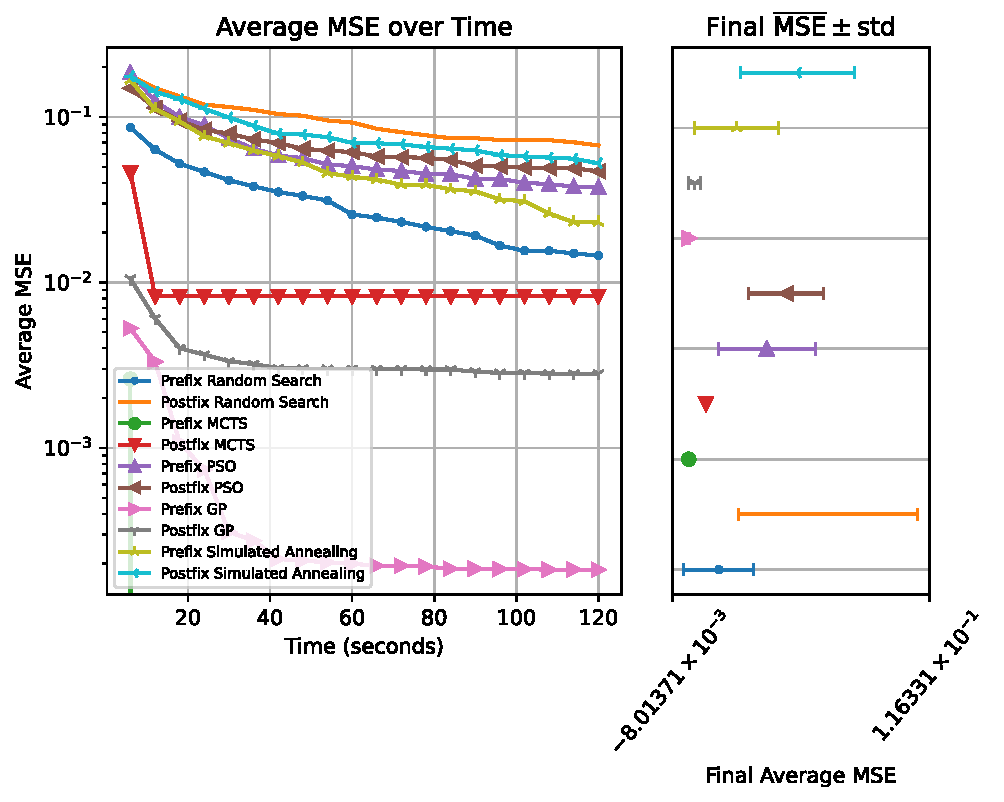
\includegraphics[width=\linewidth, keepaspectratio]{Hemberg_Benchmarks/Hemberg_Benchmark_1.pdf}
        \caption{Hemberg 1}
        \label{subfig:hemberg_1}
    \end{subfigure}
    % \hfill
    \begin{subfigure}[b]{0.49\textwidth}
        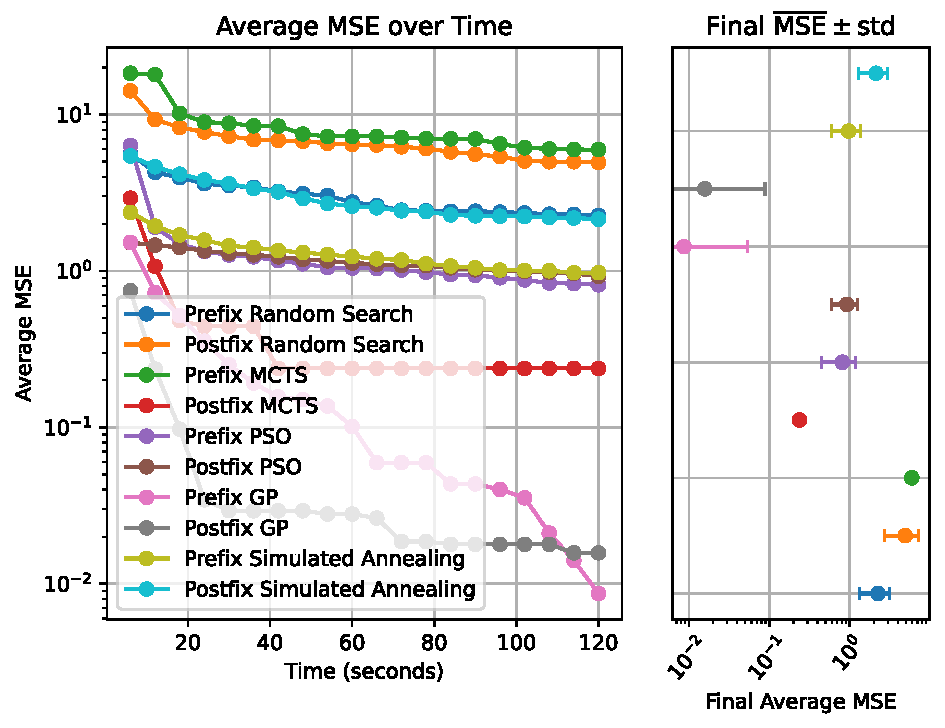
\includegraphics[width=\linewidth, keepaspectratio]{Hemberg_Benchmarks/Hemberg_Benchmark_2.pdf}
        \caption{Hemberg 2}
        \label{subfig:hemberg_2}
    \end{subfigure}
    \vspace{0.4cm}
    % \hfill
    
    \begin{subfigure}[b]{0.49\textwidth}
        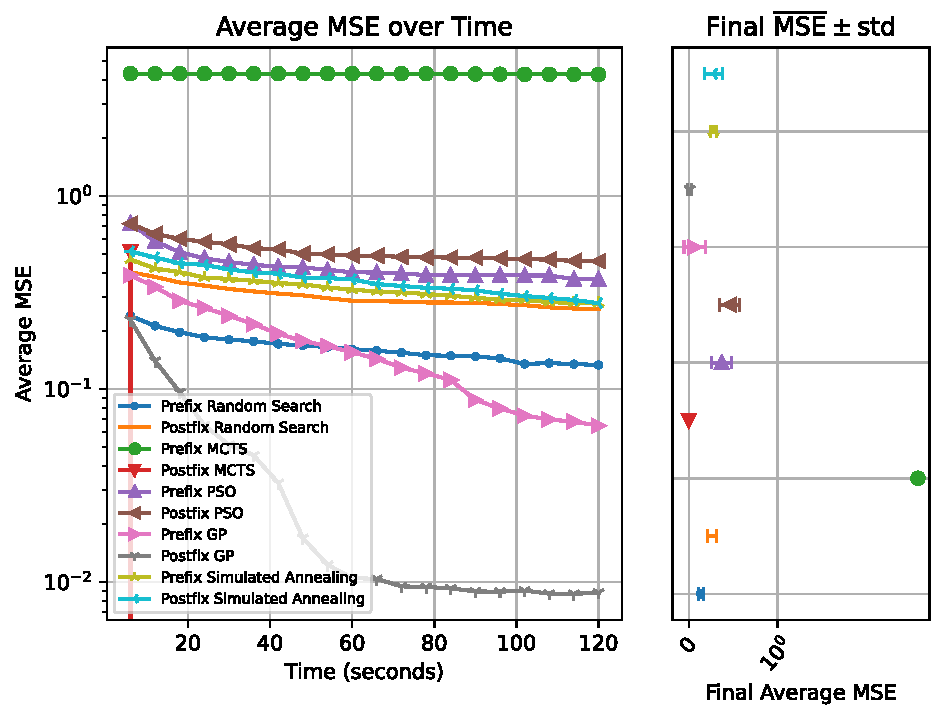
\includegraphics[width=\linewidth, keepaspectratio]{Hemberg_Benchmarks/Hemberg_Benchmark_3.pdf}
        \caption{Hemberg 3}
        \label{subfig:hemberg_3}
    \end{subfigure}
    % \vspace{0.4cm}
    % \hfill
    \begin{subfigure}[b]{0.49\textwidth}
        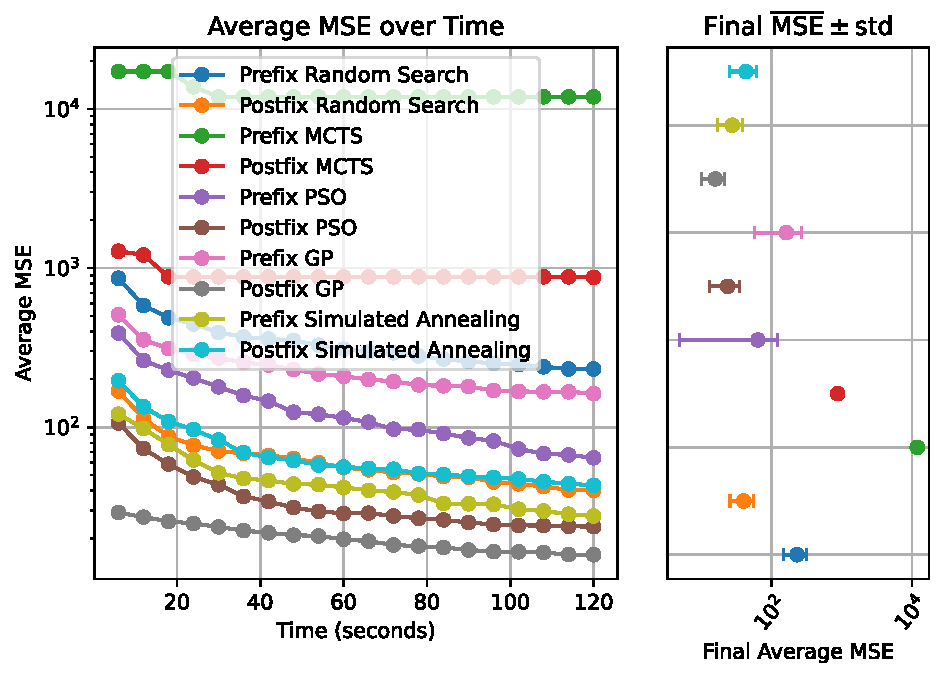
\includegraphics[width=\linewidth, keepaspectratio]{Hemberg_Benchmarks/Hemberg_Benchmark_4.pdf}
        \caption{Hemberg 4}
        \label{subfig:hemberg_4}
    \end{subfigure}
    
    \vspace{0.4cm}
    % \hfill
    \begin{subfigure}[b]{0.49\textwidth}
        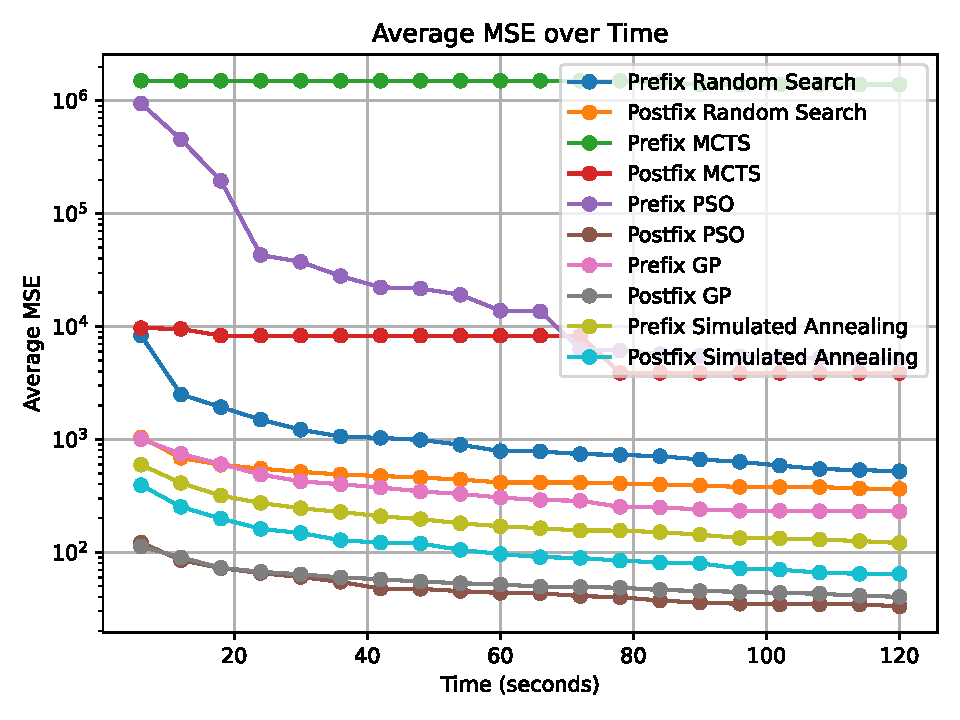
\includegraphics[width=\linewidth, keepaspectratio]{Hemberg_Benchmarks/Hemberg_Benchmark_5.pdf}
        \caption{Hemberg 5}
        \label{subfig:hemberg_5}
    \end{subfigure}
    
    \caption{Hemberg Benchmark Equations 1-5 (from Table \ref{tab:Hemberg2008PreIP_results}). Left subplots: Average MSE over 50 runs of 2 minutes each. Right Subplots: Final Average MSE $\pm$ 1 standard deviation after 2 minutes.}
    \label{fig:Hemberg_Benchmarks}
\end{figure}

\subsection{Feynman Benchmarks} \label{subsec:FeynmanBenchmarks}
In this section, we consider 5 equations from the \href{https://space.mit.edu/home/tegmark/aifeynman.html}{Feynman Symbolic Regression Database}\footnote{For a glossary of the ``Feynman Symbolic Regression Database'' Expression Trees, see \href{https://edfink234.github.io/AIFeynmanExpressionTrees/AIFeynmanExpressionTrees/AIFeynmanExpressionTrees}{here}.}, tabulated in Table \ref{tab:AI_Feynman_Benchmark_Equations} along with the depth $N$ of their expression trees that we run the benchmarks with. As in \cite{udrescu2020ai}, we randomly sample $10^5$ data points from the benchmark expressions with input variable ranges set to $[1, 5]$. The considered operators and operands are $\sin$, $\sqrt{\phantom{1}}$, $\cos$, $+$, $-$, $\cdot$, $/$, \specialcaret, and $\mathrm{const}$, input features, respectively. The results are shown in Figure \ref{fig:Feynman_Benchmarks}.

\begin{table} %TODO: when you change the refs in the `Result Plot` column, make each entry correspond to the line-color in the referenced plot
    \centering
    \scalebox{0.82}{
    \begin{tabular}{|l|l|l|l|l|l|}
\hline 
\# & Expression & Expression Tree & Depth $N$ & \# of Inputs & Result Plot \\ \hline 
  1 &  $x = \frac{q\cdot E_f}{m\cdot \left(\omega_0^2 - \omega^2\right)}$ &  \href{https://edfink234.github.io/AIFeynmanExpressionTrees/AIFeynmanExpressionTrees/AIFeynmanExpressionTrees\#figcaption61}{Feynman 1} & 4 & 5 & Figure \ref{subfig:feynman_1}  \\[0.2cm]
   2 & $F = \frac{G\cdot m_1 \cdot m_2}{\left(x_2 - x_1\right)^2 + \left(y_2 - y_1\right)^2 +\left(z_2 - z_1\right)^2}$ & \href{https://edfink234.github.io/AIFeynmanExpressionTrees/AIFeynmanExpressionTrees/AIFeynmanExpressionTrees\#figcaption5}{Feynman 2} & 5 & 9 & Figure \ref{subfig:feynman_2} \\[0.2cm]
 3 & $A = \left(\frac{Z_1 \cdot Z_2 \cdot \alpha \cdot \hbar \cdot c}{4\cdot E_n \cdot \sin^2\left(\theta/2\right)}\right)^2$ &  \href{https://edfink234.github.io/AIFeynmanExpressionTrees/AIFeynmanExpressionTrees/AIFeynmanExpressionTrees\#figcaption101}{Feynman 3} & 6 & 7 & Figure \ref{subfig:feynman_3} \\[0.2cm]
 4 &   $f = \frac{\mu_m\cdot H}{k_b \cdot T} + \frac{\mu_m\cdot \alpha}{\epsilon \cdot c^2 \cdot k_b \cdot T} \cdot M$ & \href{https://edfink234.github.io/AIFeynmanExpressionTrees/AIFeynmanExpressionTrees/AIFeynmanExpressionTrees\#figcaption82}{Feynman 4} & 7 & 8 & Figure \ref{subfig:feynman_4} \\[0.2cm]
 5 &   $k = \frac{m \cdot k_G}{L^2}\cdot \left(1+\sqrt{\left(1+\frac{2 \cdot E_n \cdot L^2}{m\cdot k_G^2}\right)}\cdot \cos\left(\theta_1-\theta_2\right)\right)$ & \href{https://edfink234.github.io/AIFeynmanExpressionTrees/AIFeynmanExpressionTrees/AIFeynmanExpressionTrees\#figcaption102}{Feynman 5} & 8 & 6 & Figure \ref{subfig:feynman_5} \\[0.2cm] \hline
\end{tabular}}
    \caption{Expressions from \cite{udrescu2020ai} considered in section \ref{subsec:FeynmanBenchmarks}.}
    \label{tab:AI_Feynman_Benchmark_Equations}
\end{table}

\begin{figure}
    \centering
    
    \begin{subfigure}[b]{0.49\textwidth}
        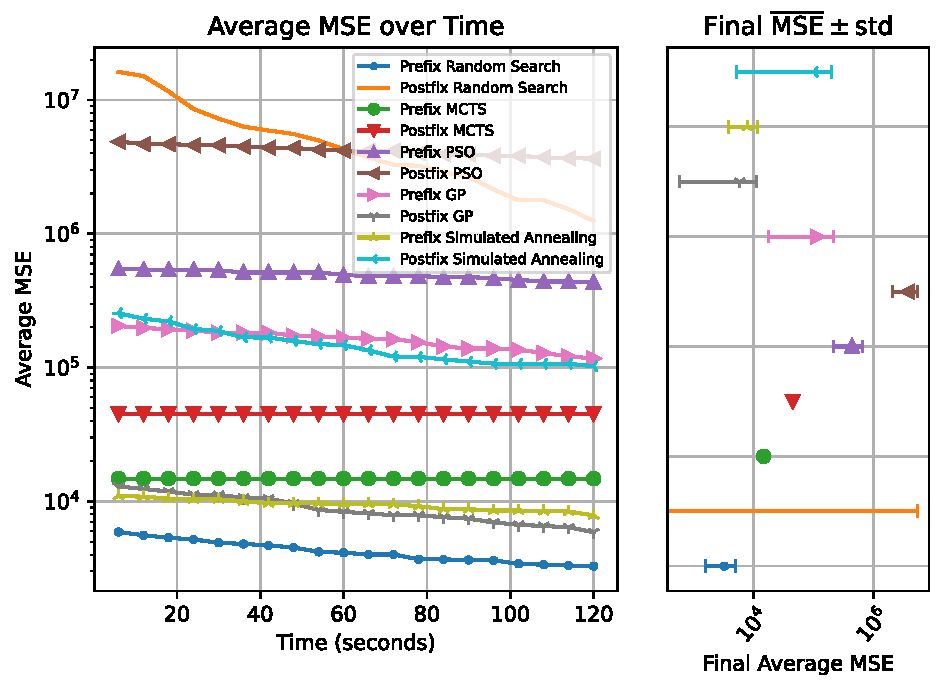
\includegraphics[width=\linewidth, keepaspectratio]{AIFeynman_Benchmarks/Feynman_Benchmark_1.pdf}
        \caption{Feynman 1}
        \label{subfig:feynman_1}
    \end{subfigure}
    % \hfill
    \begin{subfigure}[b]{0.49\textwidth}
        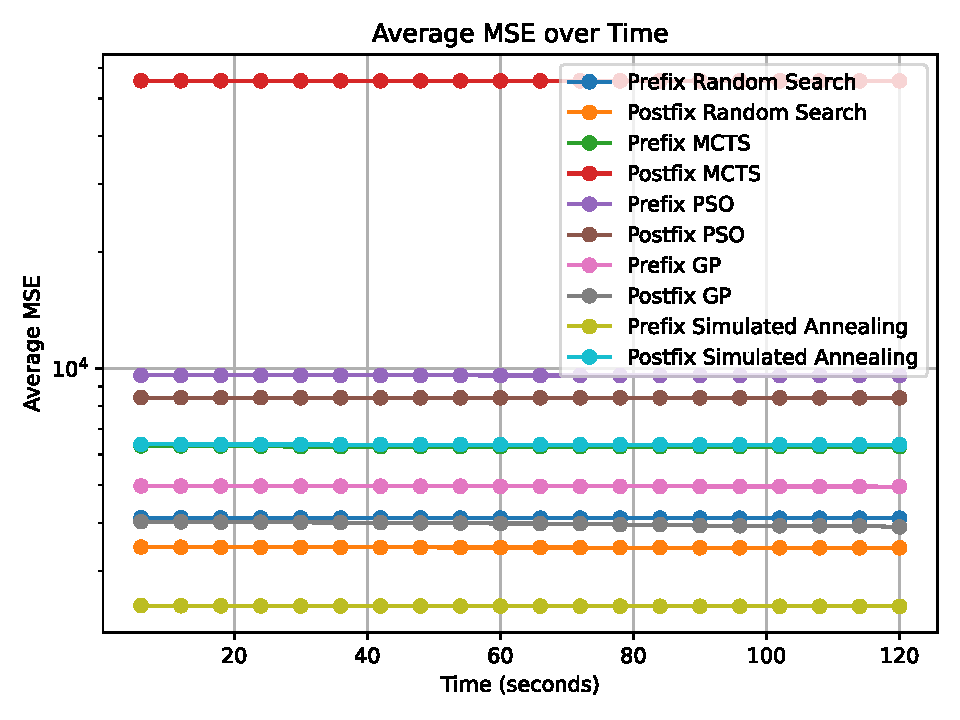
\includegraphics[width=\linewidth, keepaspectratio]{AIFeynman_Benchmarks/Feynman_Benchmark_2.pdf}
        \caption{Feynman 2}
        \label{subfig:feynman_2}
    \end{subfigure}
    
    \vspace{0.5cm}
    
    \begin{subfigure}[b]{0.49\textwidth}
        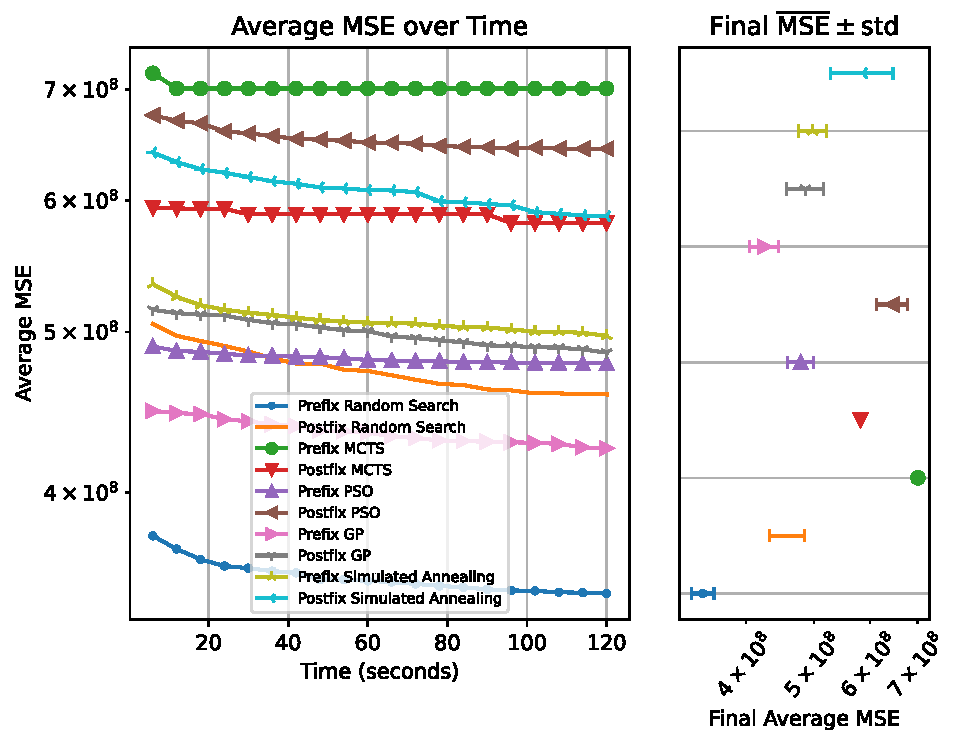
\includegraphics[width=\linewidth, keepaspectratio]{AIFeynman_Benchmarks/Feynman_Benchmark_3.pdf}
        \caption{Feynman 3}
        \label{subfig:feynman_3}
    \end{subfigure}
    % \hfill
    \begin{subfigure}[b]{0.49\textwidth}
        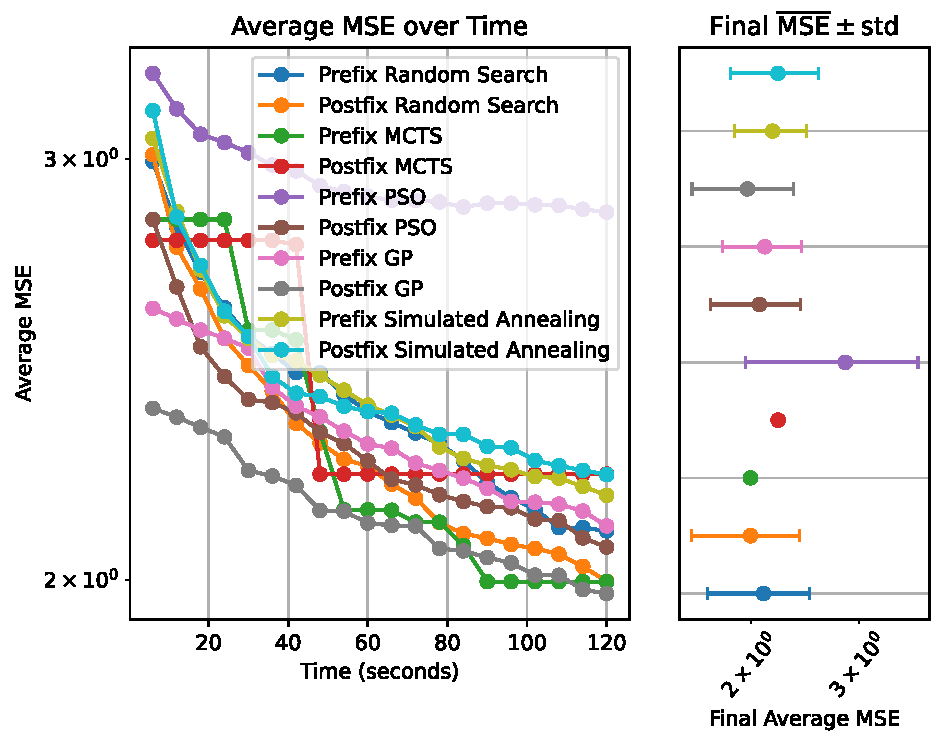
\includegraphics[width=\linewidth, keepaspectratio]{AIFeynman_Benchmarks/Feynman_Benchmark_4.pdf}
        \caption{Feynman 4}
        \label{subfig:feynman_4}
    \end{subfigure}
    
    \vspace{0.5cm}
    
    \begin{subfigure}[b]{0.49\textwidth}
        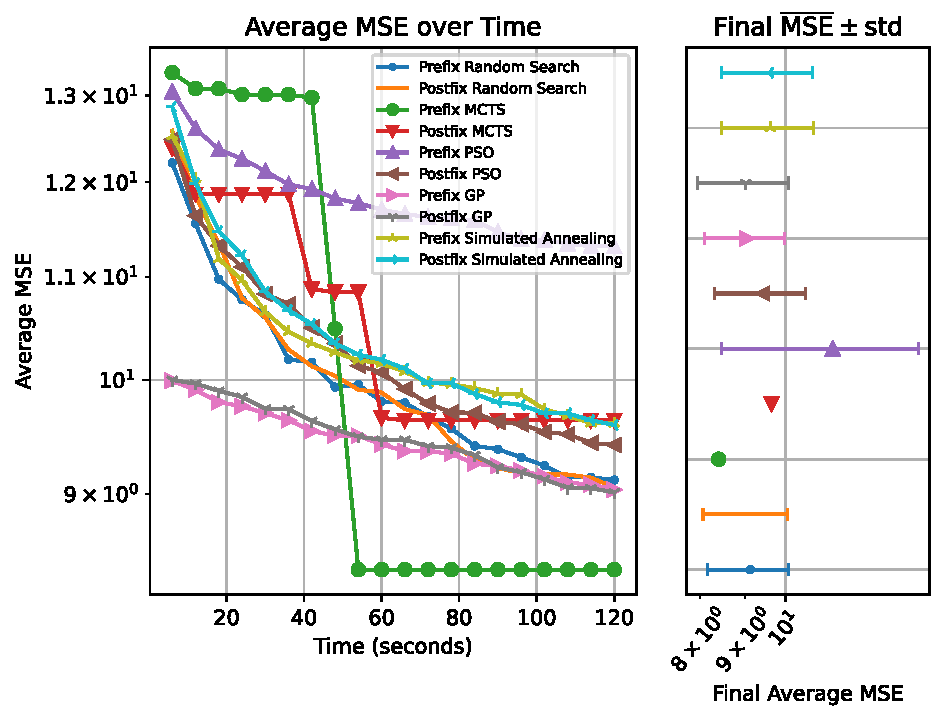
\includegraphics[width=\linewidth, keepaspectratio]{AIFeynman_Benchmarks/Feynman_Benchmark_5.pdf}
        \caption{Feynman 5}
        \label{subfig:feynman_5}
    \end{subfigure}
    
    \caption{Feynman Benchmark Equations 1-5 (from Table \ref{tab:AI_Feynman_Benchmark_Equations}). Left subplots: Average MSE over 50 runs of 2 minutes each. Right Subplots: Final Average MSE $\pm$ 1 standard deviation after 2 minutes.}
    \label{fig:Feynman_Benchmarks}
\end{figure}

\section{Remarks}

Figures \ref{fig:Hemberg_Benchmarks} and \ref{fig:Feynman_Benchmarks} show the varying performance of prefix vs postfix. To know when to use prefix and/or postfix, we build a decision tree based on the SR algorithm, the depth of the expression tree, number of input variables, and tree shape.
\par Figure \ref{fig:PrefixPostfixDecisionTree} shows that postfix $\sim$  outperforms prefix for ground-truth expression trees with larger number of nodes per layer, while prefix performs $\sim$ better on thinner trees with larger ground-truth arity or when not using Random Search.

\begin{figure}
    \centering
    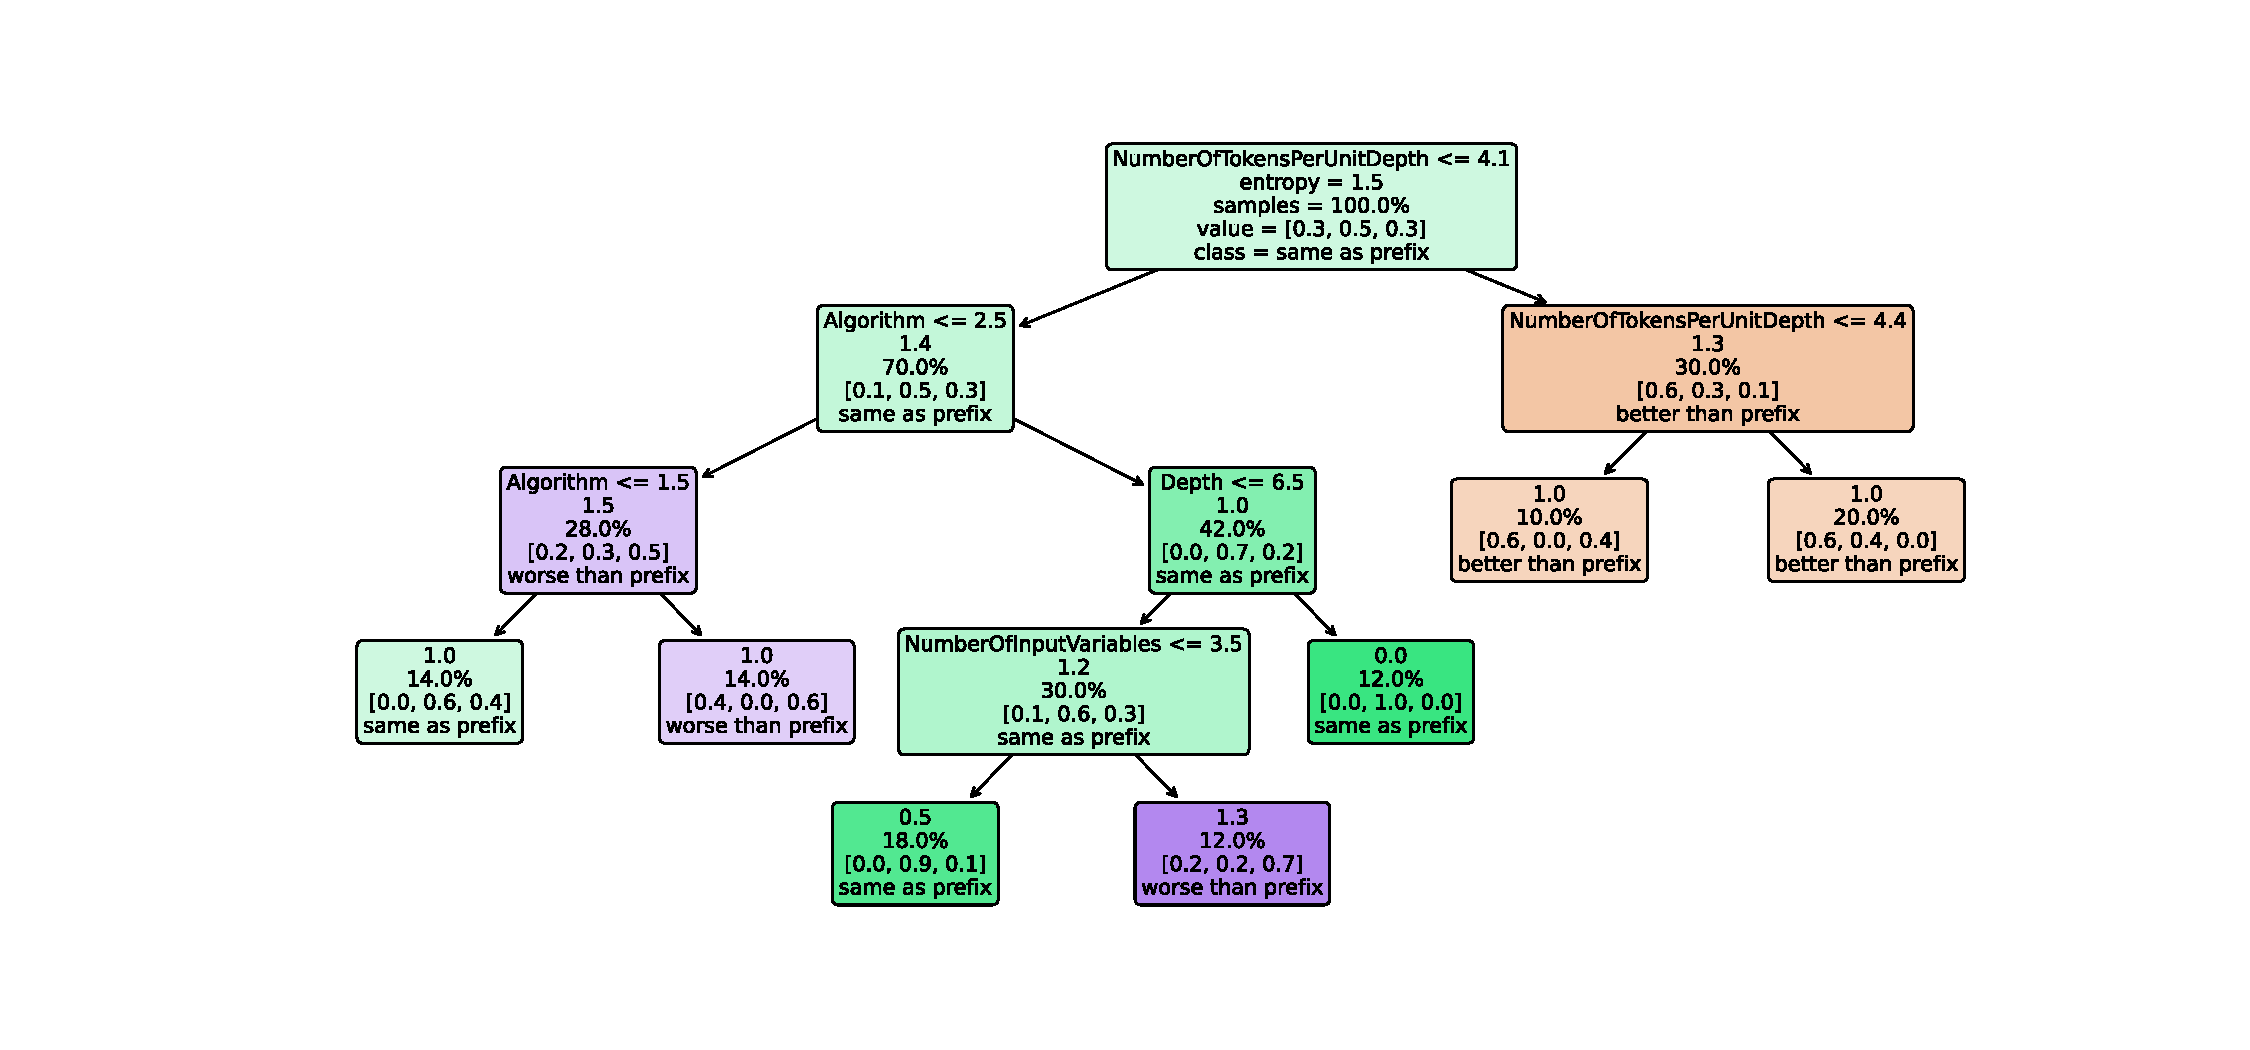
\includegraphics[width=\linewidth]{PrefixPostfixDecisionTree.pdf}
    \caption{Decision Tree for determining how postfix will perform relative to prefix. The algorithm enumeration is \texttt{\{1: `Random Search', 2: `MCTS', 3: `PSO', 4: `GP', 5: `Simulated Annealing'\}}. This decision tree classifies the data obtained in section \ref{sec:Results} with 70 \% accuracy. The code can be found \href{https://github.com/edfink234/Alpha-Zero-Symbolic-Regression/blob/0b5b6d0b56c2d108dda023a337edeb1084436da7/PrefixPostfixDecisionTree.py}{here}. } 
    \label{fig:PrefixPostfixDecisionTree}
\end{figure}

\section{Conclusion and Outlook}
In this work, we developed string-based grammars for generating symbolic expressions. These grammars elicit faultless prefix and postfix expressions corresponding to fixed-depth trees. With these grammars, we outlined five symbolic regression algorithms and benchmarked them on expressions from \cite{hemberg2008pre} and \cite{udrescu2020ai} within a C++/Eigen framework. The results suggest that postfix has greater aptitude for discovering ground truth expressions with more nodes per layer, and vice versa for prefix notation. Future work could explore how machine learning can predict the optimal expression representation from data and prior knowledge. Another extension could be implementing a fixed-depth option in existing SR frameworks to focus computational resources on searching the space of fixed-depth expressions instead of the larger space of depth $\leq$ max-depth expressions. 

\bibliographystyle{splncs04}
\bibliography{PrefixPostfixPaper}

% \appendix
% \section{Hardware Specifications}
% The benchmarks were run on a MacBook Pro with an M1 Core and $\sim$ 16 GB of usable RAM, namely, \texttt{sysctl -a | grep hw.memsize} gives: 
% \begin{verbatim}
% hw.memsize: 17179869184
% hw.memsize_usable: 16383606784
% \end{verbatim}
% The macOS system version information is obtained with \texttt{sw\_vers}:
% \begin{verbatim}
% ProductName:		macOS
% ProductVersion:		14.2.1
% BuildVersion:		23C71
% \end{verbatim}
\end{document}
